\documentclass{school-22.211-notes}
\date{March 19, 2012}

\begin{document}
\maketitle

\lecture{Diffusion Theory}
This class would not require derivation of the transport theory. 
\topic{Derivation Of Diffusion Theory From Transport Theory}
\begin{enumerate}
\item Start from the steady state continuous energy transport equation: 

\item Expand scattering source/flux in spherical harmonics, integrate over angle,


The scattering kernel is nasty, because a) $\Sigma_s$ depends on energy, hence we have to integrate over all energy; b) $\Sigma_s$ depends on angle, hence we have to integrate over all angle; c) $\Sigma_s$ depends on isotope, hence we have to integrate over all isotopes. 

\item Simplify terms: 


\item We obtain the balance equation:

Source equals sink. Notice this equation is exact so far. But since we do not know what $\vec{J}$ is, we need to approximate it somehow. 

\item Start from transport equation again, multiple by $\Omega$ and integrate over all angles: 


\item Simplify terms:



\item We obtain the net current equation:


\item We assume the source is isotropic, then the source term goes away:

\item We assume the scattering is isotropic in the Lab system, then the scattering kernel goes away:


Notice this assumption is not very good in a typical PWR -- because hydrogen scattering dominates, and hydrogen scatters isotropically in the COM system, not in the lab system. 

\item Correction term: \hi{transport correction $P_0$} approximation: 

\end{enumerate}



\topic{Multi-Group Diffusion Theory}
The diffusion coefficient approximation table is very important: $\frac{1}{3\Sigma_t}$ is off by a factor of 3! 





\clearpage
%%%%%%%%%%%%%%%%%%%%%%%%% Qualify Exam Start %%%%%%%%%%%%%%%%%%%%%%%%%%%%
\lecture{Facts For Qualify Exam}
\topic{Basics}
\begin{enumerate}
\item Common units, see Table~\ref{units}.
\begin{table}
  \centering
  \begin{tabular}{|c|c|c|c|} \hline
   $\sigma$ & $\Sigma$ & $\phi = nv$ & $R = \phi \Sigma$  \\ \hline
   $\cm^2$ & $1/\cm$ & $\frac{n}{\cm^2 \s}$ & $\frac{\mathrm{reactions}}{\cm^3 \s}$ \\ \hline
  \end{tabular}
  \caption{Units of Common Terms} \label{units}
\end{table}
\item Fast flux in hydrogen is around $10^{14}$ n/cm$^2$s, and on the order of $10^{12}$n/cm$^2$s for thermal flux. 
\item Average fission neutron energy: 2 MeV; average peak fission energy: 1 MeV; see fission sepctrum. 
\item Core decay heat after 1 day is about 1\% rated. 
\item Constants to know: 1u = 931.5 MeV. 
\item The effect of U238 energy self-shielding is about an effect of 10, that is, going from infinite dilution to U/I = 0.1. 
\end{enumerate}

\topic{Cross Section}
\begin{enumerate}
\item* If the neutron cross section is independent of energy at 0K, at 1200K the cross section would have a 1/v energy shape because of thermal motion. 
  
\item* Resonance absorption cross section dominates resonance scattering cross section most of the time (except U238). 

\item* Fission cross section: U235 fission xs at 0.1 eV and 300K is about 200 barns (200-300 barns); Pu239 fission xs is about 475 barns (380-570 barns). Hence in thermal reactors, Pu absorption should be about twice that of uranium. 

\item Elastic scattering cross section as in Figure~\ref{scatter-xs}
\begin{figure}
  \centering
  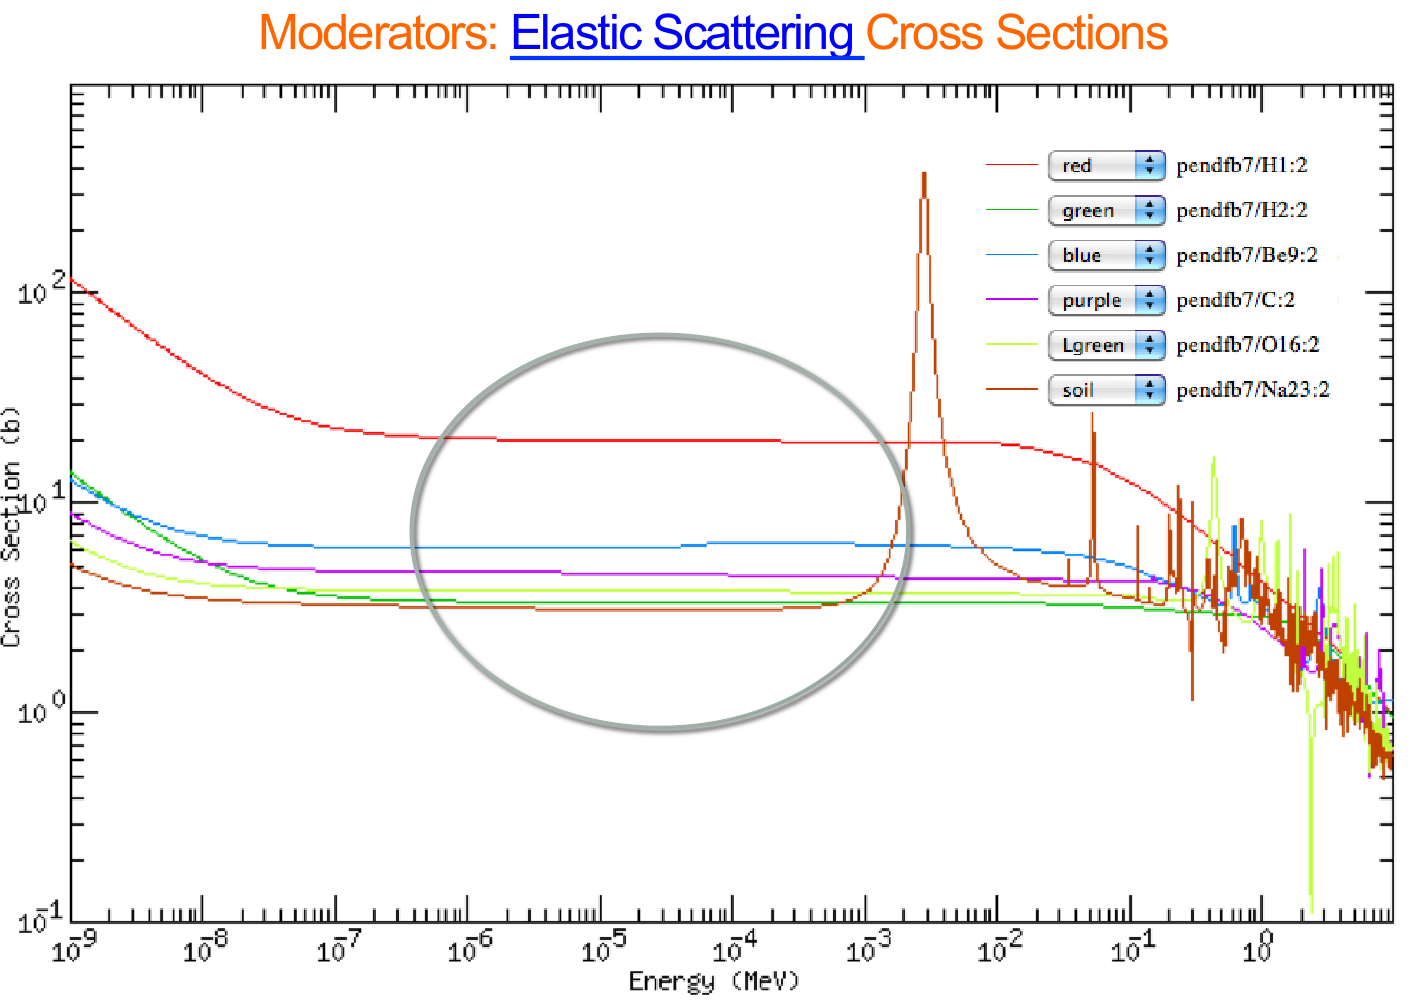
\includegraphics[width=6in]{images/intro/scatter-xs-moderator.png}
  \\
  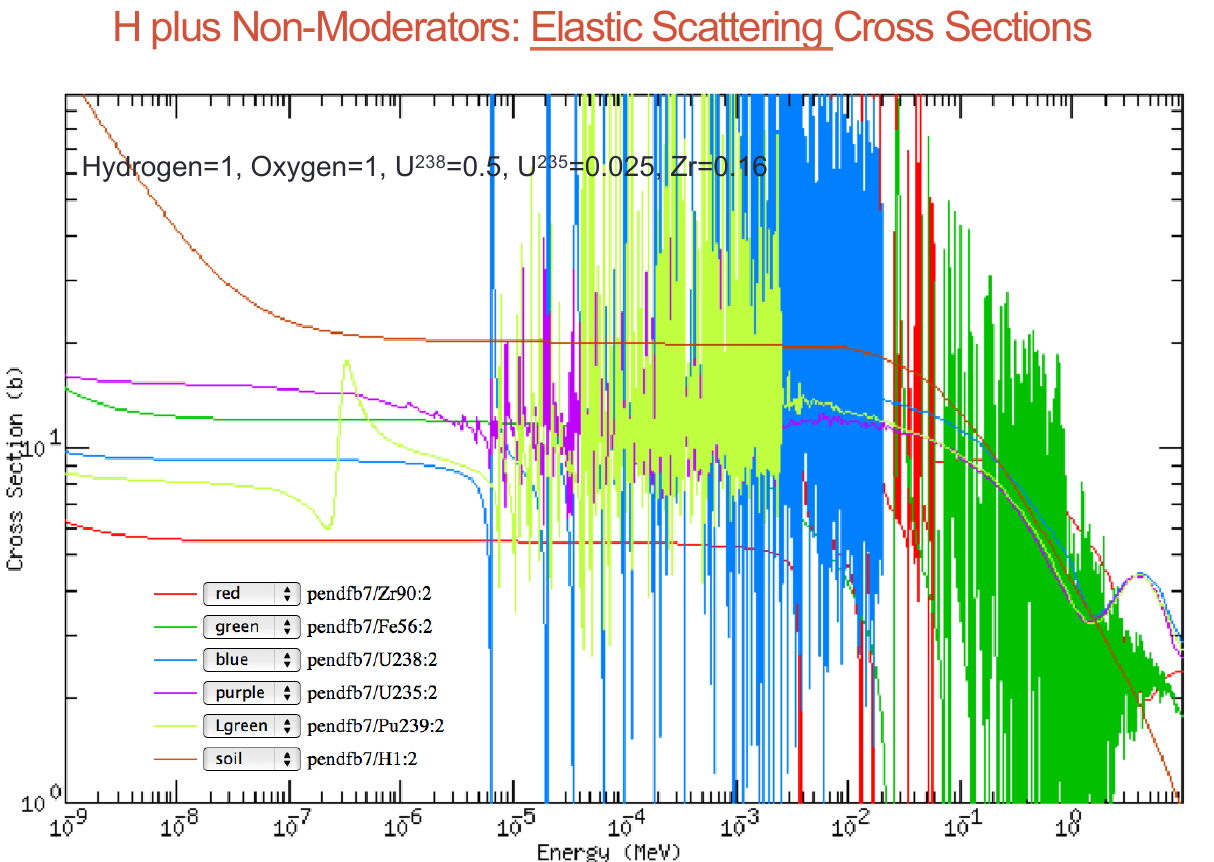
\includegraphics[width=6in]{images/intro/scatter-xs-LWR.png}
  \caption{Elastic Scattering Cross Sections} \label{scatter-xs}
\end{figure}

\item Capture cross section as in Figure~\ref{capture-xs}: 
  \begin{figure}
    \centering
    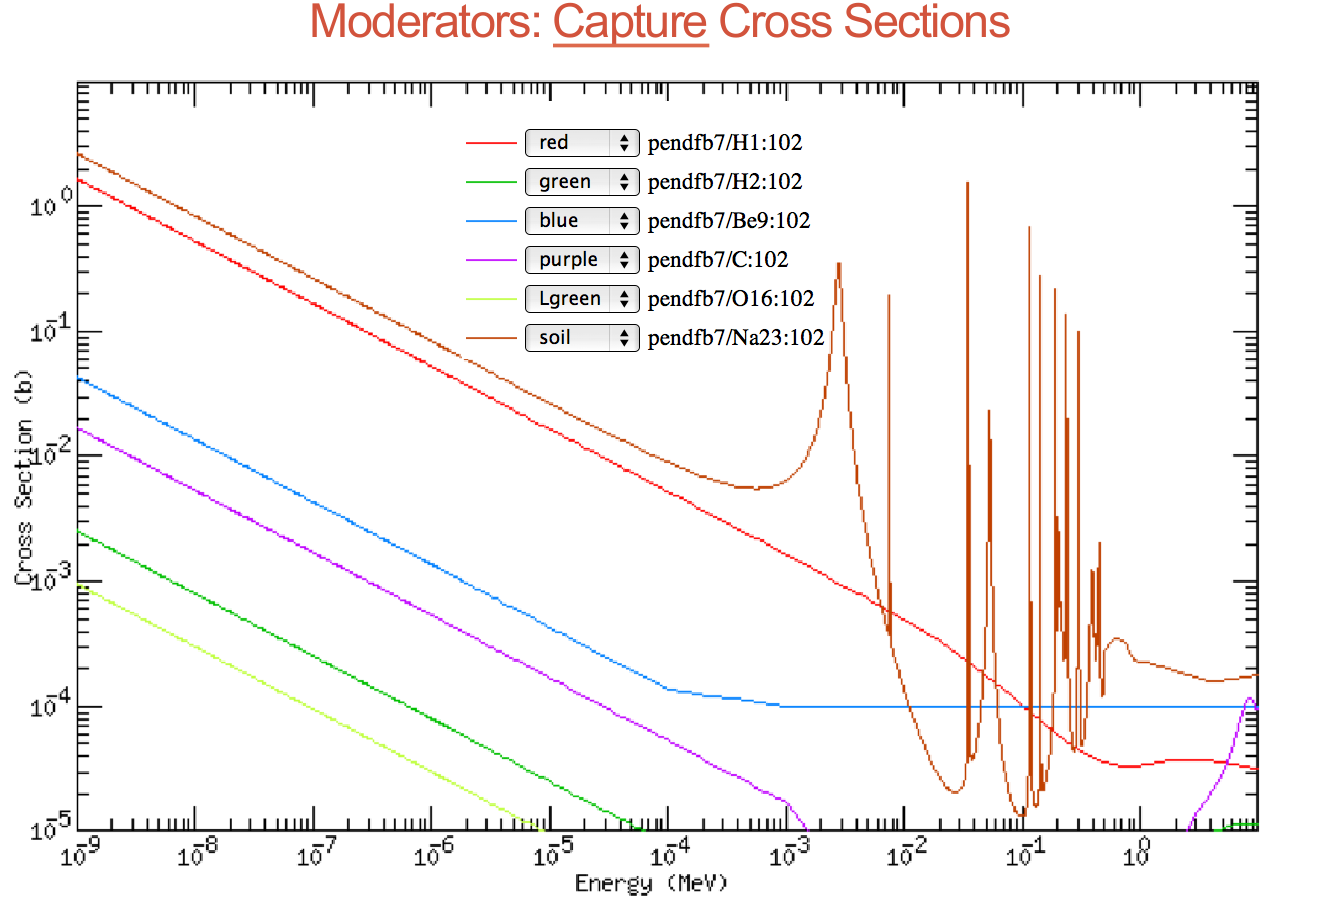
\includegraphics[width=6in]{images/intro/capture-xs.png}
    \\
    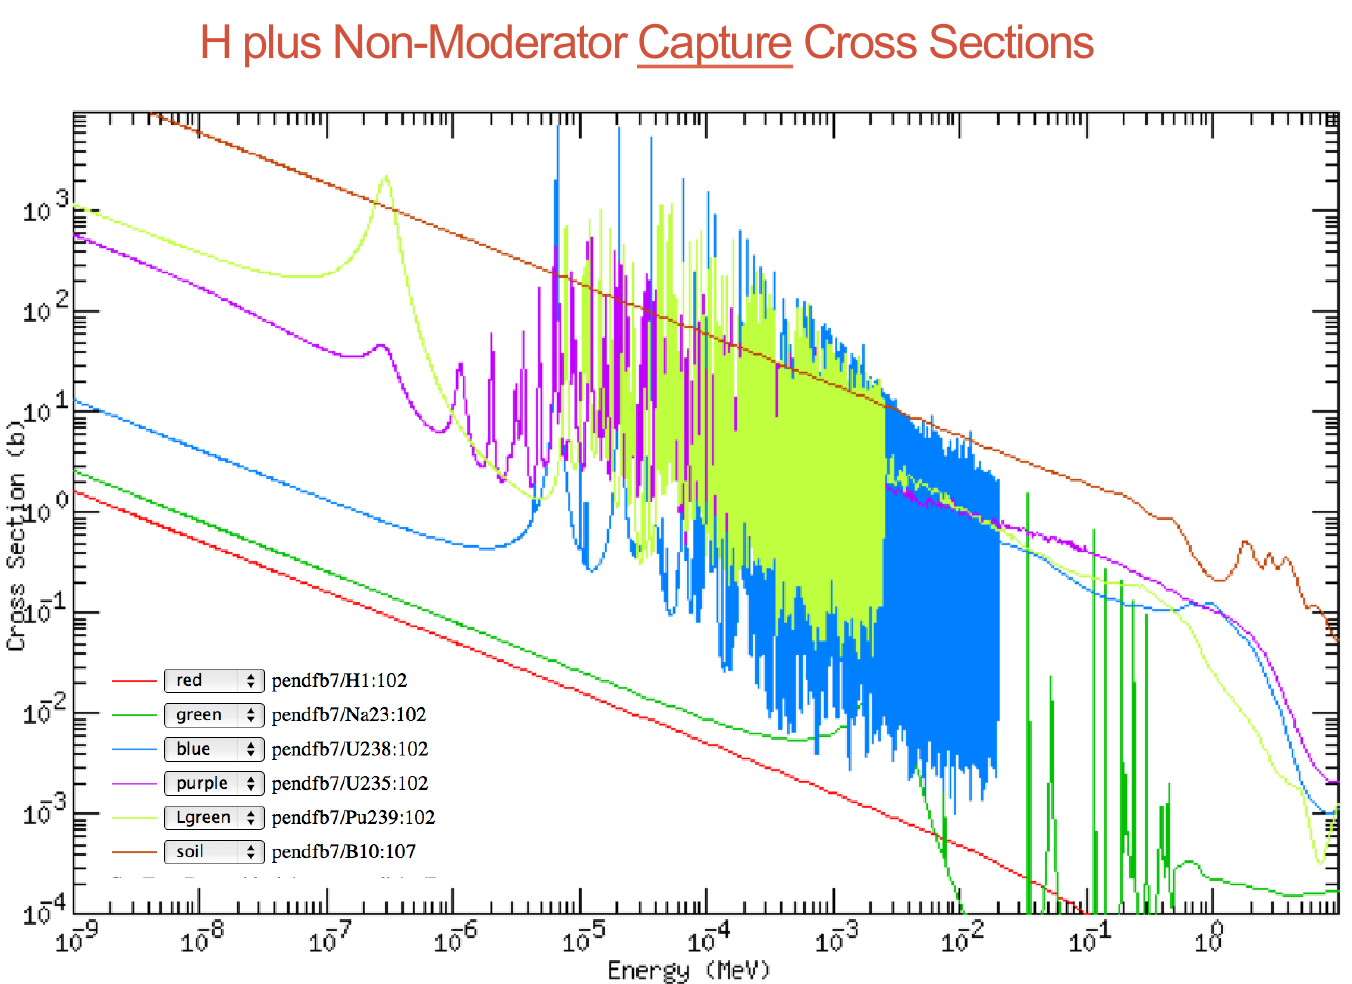
\includegraphics[width=6in]{images/intro/capture-xs-2.png}
    \caption{Capture Cross Section} \label{capture-xs}
  \end{figure}
  \begin{enumerate}
  \item H has no resonance; it has the highest scattering xs in LWR, so we can ignore any other isotopic's neutron scattering.   
  \item Na has a huge resonance in 23 keV, and more resonances at higher energies because it is a heavy isotope.
  \item Near zero energy,
    \eqn{ \sigma(E\to 0) \propto \sqrt{\frac{kT}{AE}}    }
  \item Resonance at 6 to 7 eV: U238. 
  \item U235's thermal elastic xs is larger than 238's, and they both have resonance around the same range.   
  \item A small resonance at .3 eV: Pu239 (its signiture is a super low energy scattering xs). 
  \end{enumerate}

\item Given an unknown material type, all we care is to count the nucleus density of each material and look at it's xs. 
\end{enumerate}

\topic{Kinetics}
\begin{enumerate}
\item PWR 300 pcm/K (Lec10 p. 17, FIXME). 


\item One group k-infinity: in one group $k_{\infty}$ only depends on cross sections $k_{\infty} = \frac{\nu \Sigma_f}{\Sigma_a}$ and has no flux dependency. The flux is buried in the calculation of cross section.
\item Two group k-infinity: we start with neutron balance equation:
\begin{align}
\frac{\nu \Sigma_{f1}}{k_{\infty}} \Phi_1 - \Sigma_{a1} \Phi_1 - \Sigma_{s12} \Phi_1 + \frac{\nu \Sigma_{f2}}{k_{\infty}} \Phi_2 + \Sigma_{s21} \Phi_2 &= 0 \\
\Sigma_{s12} \Phi_1 - \Sigma_{s21} \Phi_2 - \Sigma_{a2} \Phi_2 &= 0 
\end{align}
Typically what we do is to write it in a matrix form and solve for a coupled system. But even better, we can define the \hi{effective removal rate} $\bar{\Sigma}_{s12}$, and re-write the two-group balance equation: 
\begin{align}
\frac{\nu \Sigma_{f1}}{k_{\infty}} \Phi_1 - \Sigma_{a1} \Phi_1 - \bar{\Sigma}_{s12} \Phi_1 + \frac{\nu \Sigma_{f2}}{k_{\infty}} \Phi_2 &= 0 \\
\bar{\Sigma}_{s12} \Phi_1- \Sigma_{a2} \Phi_2 &= 0 
\end{align}
Then we can solve for $\frac{\Phi_1}{\Phi_2}$ from the second equation in terms of cross section, plug in the first equation, and get $k_{\infty}$ from there. Notice that we only know the relative magnitude of $\Phi$ and $\Phi_2$. 


\end{enumerate}
%%%%%%%%%%%%%%%%%%%%%%%%% Qualify Exam End %%%%%%%%%%%%%%%%%%%%%%%%%%%%


\end{document}
